% Please compile using lualatex
% Looks better with Mozilla's font "Fira" installed (https://github.com/mozilla/Fira/)
\documentclass[xcolor = dvipsnames, notheorems, 10pt]{beamer}
\usepackage{amssymb}
\usepackage{amsmath}
\usepackage{mathtools}
\usepackage{enumitem}
\usepackage{graphicx}
\usepackage{mathrsfs}
\usepackage[ngerman]{babel}
\usepackage{algorithm, algorithmic}
\usepackage{verbatim}

\title{Methoden der Numerik}
\date{\today}
\author{Christina Eilers, Julian Lüken}
\institute{Mathematisches Institut Göttingen}

\usetheme[numbering=none]{metropolis}
\renewcommand{\emph}[1]{\textcolor[HTML]{EB801A}{#1}}
\newcommand{\qedcolor}[1]{\textcolor[HTML]{22373A}{#1}}
\setbeamercolor{section in head/foot}{fg=normal text.bg, bg=structure.fg}
\setbeamercovered{transparent}

\setenumerate{align=left, leftmargin=*}
\setitemize{align=left, leftmargin=*, label=\emph{$\bullet$}}

\DeclareMathOperator{\rel}{\sim_R}

\newcommand{\vth}{\vspace{4pt}}
\theoremstyle{definition}
\newtheorem{definition}	{Definition:\vth}
\newtheorem{example}	{Beispiel:\vth}
\newtheorem{theorem}	{Satz:\vth}
\newtheorem{corollary}	{Korollar:\vth}
\newtheorem{remark}		{Bemerkung:\vth}

\renewenvironment{proof}[1][Beweis. ]{\setbeamercovered{invisible}\textbf{#1}}{\begin{flushright}\qedcolor{$\blacksquare$}\end{flushright}\setbeamercovered{transparent}}

\newenvironment{proofbegin}[1][Beweis. ]{\setbeamercovered{invisible}\textbf{#1}}

\newenvironment{proofend}{}{\begin{flushright}\qedcolor{$\blacksquare$}\end{flushright}\setbeamercovered{transparent}}


\begin{document}
% Title page
\begin{frame}
	\maketitle
\end{frame}

\section{Aufgabe 1 - Wärmegleichung}
\begin{frame}
\frametitle{Wärmegleichung}
	Die Wärmegleichung lautet
	$$ \frac{\partial u}{\partial t} - \alpha \nabla^2 u$$
	Mit $u: \Omega \times \mathbb{R}^+ \rightarrow \mathbb{R}$ mit folgenden Randbedingungen:
	\begin{itemize}
		\item $ u(x,t) = R$ für $ x \in \partial \Omega$	
		\item $ u(x,0) = f(x) $, wobei $f$ beliebig aber fest.
	\end{itemize}
\end{frame}

\begin{frame}
\frametitle{Diskretisierung der Wärmegleichung}
	Nimm endlich viele, äquidistante Stellen aus $\Omega$, sodass Folgen entstehen mit $x_i = ih + x_0$ und $y_j = jh + y_0$. Wähle zusätzlich für die Zeit $t_k = k\Delta t + t_0$ Wir schreiben $u_{i,j}^k$ für die $(i,j)$-te Stelle zum Zeitpunkt $k$. Für jedes $k \in \mathbb{N}$ entsteht eine $m \times m$ Matrix. Zum Zeitpunkt $k$ haben wir dann:
	$$
	\begin{pmatrix}
		u^k_{0,0}& 		u^k_{0,1}& \cdots & u^k_{0,m} 	\\
		u^k_{1,0}&		\ddots&			&\vdots	\\
		\vdots & & &	\\
		u^k_{m,0}&	\cdots	&			 & u^k_{m,m}
	\end{pmatrix}
	$$
\end{frame}
\begin{frame}
\frametitle{Diskretisierung der Wärmegleichung}
	Schreibe diese Matrix als Vektor, damit wir einen linearen Operator in Form einer Matrix darauf anwenden können, folgendermaßen:
	$$ u^k =
	\begin{pmatrix}
		u^k_{0,0} \\
		u^k_{0,1} \\
		\vdots \\
		u^k_{0,m} \\
		u^k_{1,0} \\
		u^k_{1,1} \\
		\vdots \\
		u^k_{m,m}
	\end{pmatrix}
	$$
\end{frame}

\begin{frame}
\frametitle{Diskretisierung}
	Aus der Taylor-Entwicklung folgt für die Ableitung nach $t$
	$$\frac{\partial u}{\partial t}(x,y,t) = \frac{u(x,y,t+\Delta t) - u(x,y,t)}{\Delta t} + O(\Delta t^2)$$
	und für den Laplace-Operator
	\begin{multline*}
		\nabla^2u(x,y,t) = \frac{1}{4h^2} \bigg(u(x-h,y,t) + u(x+h,y,t) \\+ u(x,y-h,t) + u(x,y+h,t) - 4u(x,y,t) \bigg) + O(h^4)
	\end{multline*}
	Für diese Terme können wir im diskreten Fall unter Vernachlässigung des Fehlers schreiben
	$$ \frac{u_{i,j}^{k+1} - u_{i,j}^k}{\Delta t} \quad\text{und}\quad \frac{1}{4h^2} \bigg( u_{i+1,j}^k + u_{i-1,j}^k + u^k_{i,j+1} + u^k_{i,j-1} - 4u^k_{i,j} \bigg)$$
\end{frame}


\begin{frame}
\frametitle{Explizites Euler-Verfahren}
	Sei ab jetzt $h = 1$ und $\Delta t = 1$.
	Für das explizite Euler-Verfahren suchen wir eine Matrix $A \in \mathbb{R}^{m^2 \times m^2}$ für die gilt:
	$$u^{k+1} = u^k + \alpha A u^k$$
	Mit den aus der Taylor-Entwicklung gewonnenen Diskretisierungen für unsere Differentialoperatoren erhalten wir mit ein paar Umformungen die Iterationsvorschrift
	$$u^{k+1}_{i,j} = \alpha \bigg( \frac{u_{i+1,j}^k + u_{i-1,j}^k + u^k_{i,j+1} + u^k_{i,j-1}}{4} \bigg)
		+ (1-\alpha)u^k_{i,j} $$
\end{frame}

\begin{frame}
\frametitle{Explizites Euler-Verfahren}
	Im expliziten Euler-Verfahren sieht die Verfahrensmatrix dann so aus:
	$$ A = \frac{1}{4}
		\begin{bmatrix}
			\mathbf{L} 	& \mathbf{I} 	& \mathbf{0} 	& 				& \cdots 		&				& \mathbf{0} 	\\
			\mathbf{I}	& \mathbf{L} 	& \mathbf{I} 	& 				&				& 				&			 	\\
			\mathbf{0}	& \mathbf{I}	& \mathbf{L}	& 				& 				&				&				\\
			\vdots		&				&				& 				& \ddots		&				& \vdots		\\
						&				&				&				&				&				&				\\
						&				&				&				&				& \mathbf{L}	& \mathbf{I}	\\
			\mathbf{0}	&				&				&	\cdots		&				& \mathbf{I}	& \mathbf{L}	\\		
		\end{bmatrix}
	\quad
	\text{wobei}
	\quad
	L = \text{tridiag}(1,-4,1)$$
	
	Damit wird das explizite Euler-Verfahren in unserem Fall zu
	$$ u^{k+1} = u^k + \alpha A u^k = (\alpha A + I)u^k $$
\end{frame}

\begin{frame}
\frametitle{Implizites Euler-Verfahren}
	Im impliziten Euler-Verfahren gilt es nun, eine Iterationsvorschrift der Form
	$$ u^{k+1} = u^k + \alpha Bu^{k+1} $$
	zu finden.
	Aus dem expliziten Euler-Verfahren lässt sich dafür
	$$ B = A (\alpha A + I)^{-1} $$
	herleiten.
	Wir gewinnen daraus ein Gleichungssystem in der Form $Cx = d$, welches wir in jedem Schritt nach $x$ lösen können
	$$ u^k = (I - \alpha A (\alpha A + I)^{-1}) u^{k+1} $$
	\begin{remark}
		Hierfür eignet sich das CG-Verfahren.

		Weiterhin ist das LGS nur lösbar, wenn $\alpha \neq 1$
	\end{remark}

\end{frame}

\begin{frame}
\frametitle{Finite Differenzen}
	Durch Umstellen der Wärmegleichung mit $A$ von vorhin können wir durch folgende Iterationsvorschrift mit gegebenen Startwerten $u^0$ den Verlauf der Wärmegleichung simulieren:
	$$u^{k+1} = (\alpha A+I)u^k$$
\end{frame}

\begin{frame}
\frametitle{Finite Differenzen II}
	\begin{remark}
		Wenn man $u^k$ als Matrix schreibt, so kann man ebenfalls mit $L_\alpha = 0.5 \cdot \alpha \cdot \text{tridiag}(1,-2,1) + I$ den gleichen Schritt folgendermaßen durchführen:

		$$u^{k+1} = 0.5 \big( L_\alpha u^k + u^kL_\alpha \big)$$
		Zwar werden so pro Schritt zwei Matrixmultiplikationen und eine Addition durchgeführt, allerdings nur mit $m \times m$ Matrizen statt mit $m^2 \times m^2$ Matrizen.
	\end{remark}
\end{frame}


\begin{frame}
\frametitle{Konjugierte Gradienten}
	Wir erinnern uns an das implizite Euler-Verfahren mit dem Gleichungssystem 
		$$ u^k = (I - \alpha A (\alpha A + I)^{-1}) u^{k+1} $$
	Um dieses zu lösen, definieren wir 
		$$ K = (I - \alpha A (\alpha A + I)^{-1})$$
	In jedem Schritt unserer Iteration lösen wir nun das Gleichungssystem
		$$ u^k = Ku^{k+1}$$
	mithilfe des Algorithmus der konjugierten Gradienten.

\end{frame}

\begin{frame}
\frametitle{Konjugierte Gradienten}
	Wir wählen $b = u^k$. In jedem Schritt führen wir aus
	\begin{algorithm}[H]
		\begin{algorithmic}[1]
			\STATE $x_0 \gets b$, $k \gets 0$, $r_0 \gets b-Kx_0$, $d_0 \gets r_0$
			\WHILE {$r_k^T r_k > \varepsilon$}
				\STATE $\alpha_k = \frac{r_k^T r_k}{d_k^T K d_k}$
				\STATE $x_{k+1} \gets x^k + \alpha_k d_k$
				\STATE $r_{k+1} \gets r_k - \alpha_k K d_k$
				\STATE $\beta_k \gets \frac{r_{k+1}^T r_{k+1}}{r_k^T r_k}$
				\STATE $d_{k+1} \gets r_{k+1} + \beta_k d_k$
				\STATE $k \gets k+1$
			\ENDWHILE
			\RETURN $x_k$
		\end{algorithmic}
		\caption{Konjugierte-Gradienten Verfahren}
	\end{algorithm}
\end{frame}

\begin{frame}
\frametitle{Gauss-Elimination}
	Man kann das LGS ebenfalls mit Gauss-Elimination lösen. Zunächst brauchen wir dafür die LU-Zerlegung $K = LU$, wobei $L$ untere Dreiecksmatrix und $U$ obere Dreiecksmatrix.
	\begin{algorithm}[H]
		\begin{algorithmic}[1]
			\STATE $U \gets K$, $L \gets I$
			\FOR {$i \in \{1 ... n\}$}
				\FOR {$k \in \{i+1 ... n\}$}
					\STATE $L_{ki} \gets \frac{U_{ki}}{U{ii}}$
					\FOR {$j \in \{i ... n\}$}
						\STATE $U_{kj} \gets U_{kj} - L_{ki} \cdot U_{ij}$
					\ENDFOR
				\ENDFOR
			\ENDFOR
			\RETURN $L$, $U$
		\end{algorithmic}
		\caption{LU-Zerlegung}
	\end{algorithm}
\end{frame}

\begin{frame}
\frametitle{Gauss-Elimination}
	Jetzt löst man durch Vorwärtselimination
	$$Ly = u^{k}$$
	und danach durch Rückwärtselimination
	$$Uu^{k+1} = y$$
	\begin{remark}
		Die $LU$-Zerlegung von $K$ müssen wir für unsere Zwecke nur einmal bestimmen. 
	\end{remark}

\end{frame}

\section{Aufgabe 2 - Newton-Verfahren}
\begin{frame}
\frametitle{Problemstellung}
	Löse
		$$\min_{x \in \mathbb{R}^7} \quad f(x) = \frac{1}{2}||g(x)||_2^2$$
	mit $g: \mathbb{R}^7 \rightarrow \mathbb{R}^8$, $\nabla g: \mathbb{R}^7 \rightarrow \mathbb{R}^{7 \times 8}$ und $\nabla^2 g: \mathbb{R}^7 \rightarrow \mathbb{R}^{7 \times 7 \times 8}$. $x_0 = 0$ und für die Lösung soll gelten $||\nabla f(\bar x)||_2 < 10^{-11}$
	\vfill
\end{frame}

\begin{frame}
\frametitle{Newton-Verfahren}
	Im Newton-Verfahren nutzen wir die Iterationsvorschrift
	$$x_{n+1} = x_n - (\nabla^2 f(x))^{-1}\, \nabla f(x)$$
	Oder in Pseudocode:
	\begin{algorithm}[H]
		\begin{algorithmic}[1]
			\STATE $x \gets 0 \in \mathbb{R}^7$
			\WHILE{$||\nabla f(x)||_2 \geq 10^{-11}$}
				\STATE $H_\text{inv} \gets \nabla^2 f(x)$
				\STATE $x \gets x - H_\text{inv}\nabla f(x)$ 
			\ENDWHILE
			\RETURN x
		\end{algorithmic}
		\caption{Newton-Verfahren}
	\end{algorithm}
	\begin{remark}
		Das funktioniert nur, wenn $\nabla^2 f$ existiert und bekannt ist.
	\end{remark}
\end{frame}

\begin{frame}
\frametitle{Quasi-Newton-Verfahren}
	\begin{algorithm}[H]
		\begin{algorithmic}[1]
			\STATE $x_0 \gets 0 \in \mathbb{R}^7$
			\STATE $H_0 = I$
			\STATE $p_0 = -\nabla f(x_0)$
			\STATE $k = 0$
			\WHILE{$||\nabla f(x)||_2 \geq 10^{-11}$}
				\STATE $\alpha \gets \text{argmin}_{\alpha \in \mathbb{R}}\, f(x_k + \alpha p_k)$
				\STATE $s_k \gets \alpha p_k$
				\STATE $x_{k+1} \gets x_k+s_k$
				\STATE $y_k \gets \nabla f(x_{k+1}) - \nabla f(x_k)$
				\STATE $H_k = \text{update}(H_k)$
				\STATE $k \gets k+1$
			\ENDWHILE
			\RETURN $x_k$
		\end{algorithmic}
		\caption{Quasi-Newton-Verfahren}
	\end{algorithm}
\end{frame}

\begin{frame}
\frametitle{Quasi-Newton-Updates}
	Für die Funktion update auf der letzten Folie gibt es verschiedene Möglichkeiten, beispielsweise:
	\begin{center}
		\begin{tabular}{r|l}
			BFGS 		&	$H_{k+1} = H_k + \frac{y_k y_k^T}{y_k^T s_k} + \frac{H_k s_k s_k^T H_k^T}{s_k^T H_k s_k}$\\
			& \\
			Broyden 	&	$H_{k+1} = H_k + \frac{s_k - H_k y_k}{y_k^T y_k} y_k^T$
		\end{tabular}
	\end{center}
\end{frame}


\begin{frame}
\frametitle{Lösungen}
	\footnotesize
	\begin{center}
		\begin{tabular}{r || l | l | l}
			& klassisch & BFGS & Broyden\\ \hline \hline
			$f(x)$ &$2291.020503182124$ &$2291.0205031821224$ &$2291.020503182123$\\
			$\nabla f(x)$	&$\begin{pmatrix}
													0 \\
													-1.137 \\
													0.941 \\
													-0.284 \\
													5.684 \\
													0 \\
													0
							\end{pmatrix} \cdot 10^{-13}$
							&$\begin{pmatrix}
													-2.274 \\ 
													67.075 \\
													21.245 \\
													-7.248 \\
													37.232 \\
													-2.256 \\
													-2.487
							\end{pmatrix} \cdot 10^{-13}$
							&$\begin{pmatrix}
													-3.411 \\
													-14.780 \\
													-4.814 \\
													1.705 \\
													86.118 \\
													-3.606 \\
													0.249 \\
							\end{pmatrix} \cdot 10^{-13}$\\
		\end{tabular}
	\end{center}
	\normalsize
\end{frame}
\begin{frame}
\frametitle{Hesse-Matrizen}
	\scriptsize
		$$H^{-1} = \begin{pmatrix}
			&2.151 &0.598 &3.538 &16.956 &-0.078 &-2.615 &-0.039 \\
			&0.598 &3.288 &0.121 &22.659 &0.310 &13.016 &-0.011 \\
			&3.538 &0.121 &13.622 &45.657 &-0.220 &-8.099 &-0.260 \\
			&16.956 &22.659 &45.657 &323.998 &1.294 &58.392 &-0.897 \\
			&-0.078 &0.310 &-0.220 &1.294 &0.148 &2.717 &0.001 \\
			&-2.615 &13.016 &-8.099 &58.392 &2.717 &93.675 &0.047 \\
			&-0.039 &-0.011 &-0.260 &-0.897 &0.001 &0.047 &3.256 \\
		\end{pmatrix} \cdot 10^{-3}$$
		$$H^{-1}_\text{BFGS} = \begin{pmatrix}
			&1.992 &0.337 &3.517 &14.757 &-0.068 &-3.207 &-0.025 \\
			&0.337 &2.532 &0.301 &17.282 &0.273 &10.557 &-0.003 \\
			&3.517 &0.301 &13.449 &46.290 &-0.189 &-7.443 &-0.278 \\
			&14.757 &17.282 &46.290 &284.436 &1.163 &42.147 &-0.838 \\
			&-0.068 &0.273 &-0.189 &1.163 &0.135 &2.584 &-0.014 \\
			&-3.207 &10.557 &-7.443 &42.147 &2.584 &80.445 &0.562 \\
			&-0.025 &-0.003 &-0.278 &-0.838 &-0.014 &0.562 &3.115
		\end{pmatrix} \cdot 10^{-3}$$
		$$H^{-1}_\text{Broyden} = \begin{pmatrix}
			&1.003 &0.353 &2.534 &10.787 &-0.024 &-0.808 &-0.305 \\
			&0.016 &0.559 &1.185 &4.623 &0.082 &4.472 &-0.130 \\
			&0.035 &0.129 &9.330 &30.184 &-0.035 &-1.636 &-0.773 \\
			&0.301 &4.001 &62.421 &234.475 &-0.381 &2.729 &-5.924 \\
			&-0.171 &0.436 &-1.168 &-0.179 &0.145 &2.657 &0.025 \\
			&1.258 &-0.488 &22.002 &72.069 &0.185 &7.744 &-1.962 \\
			&0.009 &-0.057 &-1.015 &-3.702 &0.007 &-0.004 &1.718
		\end{pmatrix} \cdot 10^{-3}$$
	\normalsize
\end{frame}

\begin{frame}
	\begin{center}
	\frametitle{Funktionswerte für Newton-Verfahren}
		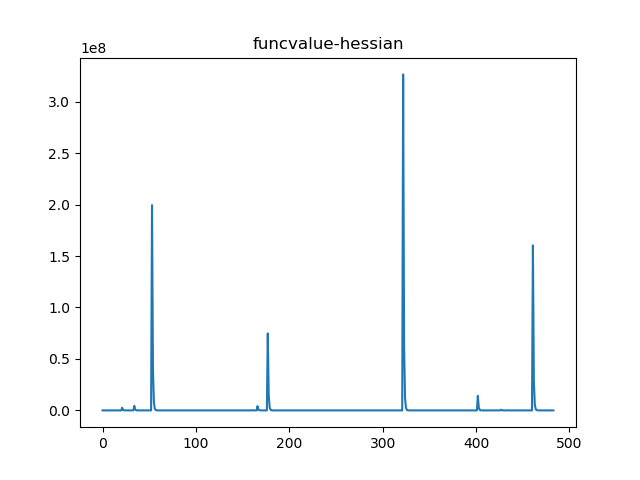
\includegraphics[width=.8\linewidth]{{c:/Users/julian/git/mdn/aufg2/funcvalue-hessian.png}}
	\end{center}
\end{frame}
\begin{frame}
\frametitle{Funktionswerte für Quasi-Newton: BFGS}
	\begin{center}
		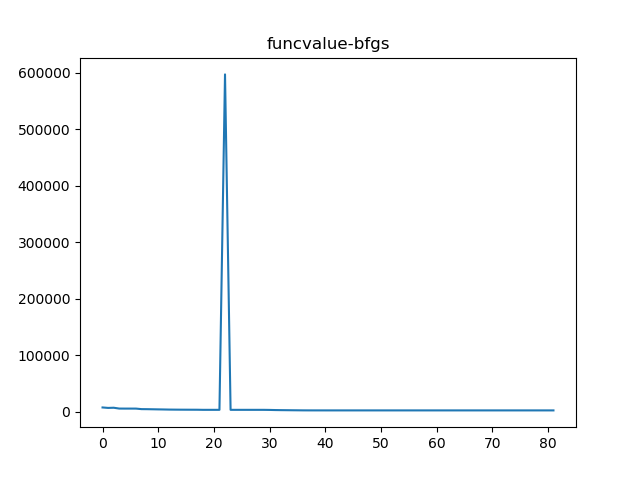
\includegraphics[width=.8\linewidth]{{c:/Users/julian/git/mdn/aufg2/funcvalue-bfgs.png}}
	\end{center}
\end{frame}
\begin{frame}
\frametitle{Funktionswerte für Quasi-Newton: Broyden}
	\begin{center}
		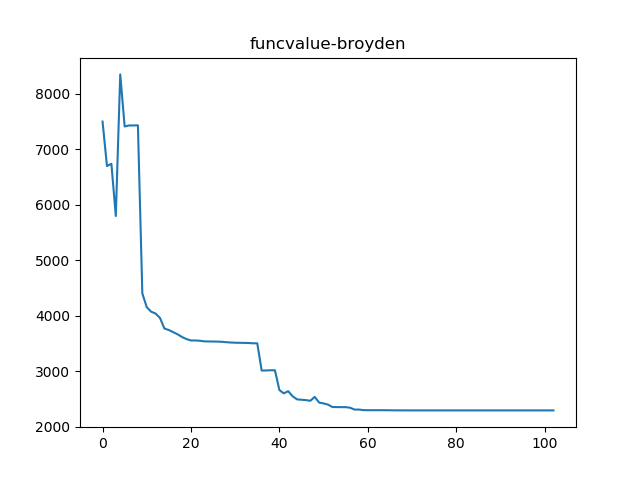
\includegraphics[width=.8\linewidth]{{c:/Users/julian/git/mdn/aufg2/funcvalue-broyden.png}}
	\end{center}
\end{frame}

\begin{frame}
	\begin{center}
	\frametitle{Grad für Newton-Verfahren}
		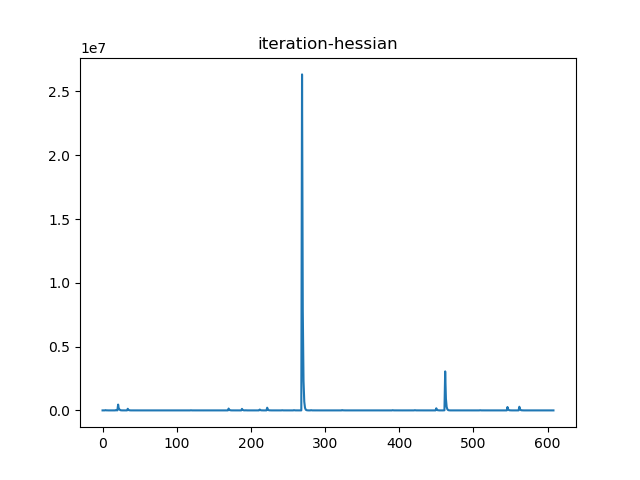
\includegraphics[width=.8\linewidth]{{c:/Users/julian/git/mdn/aufg2/iteration-hessian.png}}
	\end{center}
\end{frame}
\begin{frame}
\frametitle{Grad für Quasi-Newton: BFGS}
	\begin{center}
		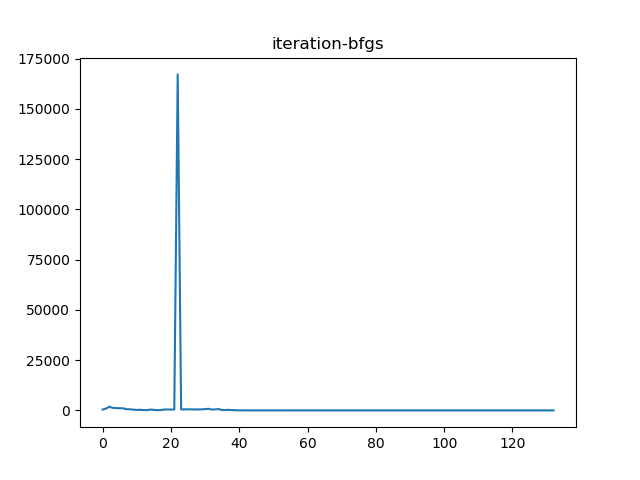
\includegraphics[width=.8\linewidth]{{c:/Users/julian/git/mdn/aufg2/iteration-bfgs.png}}
	\end{center}
\end{frame}
\begin{frame}
\frametitle{Grad für Quasi-Newton: Broyden}
	\begin{center}
		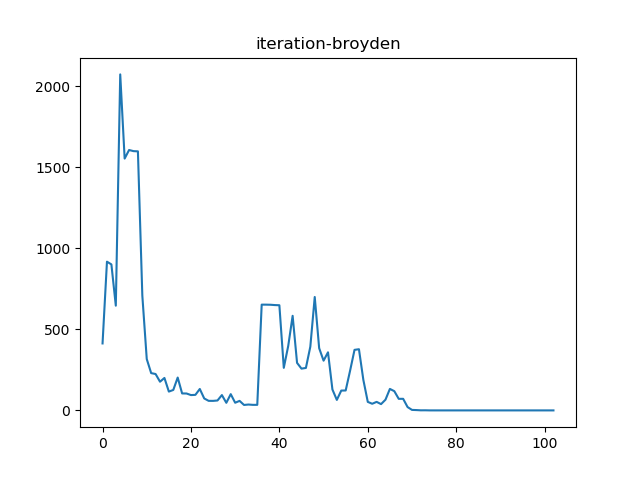
\includegraphics[width=.8\linewidth]{{c:/Users/julian/git/mdn/aufg2/iteration-broyden.png}}
	\end{center}
\end{frame}

\begin{frame}
	\begin{center}
	\frametitle{Schrittweite für Newton-Verfahren}
		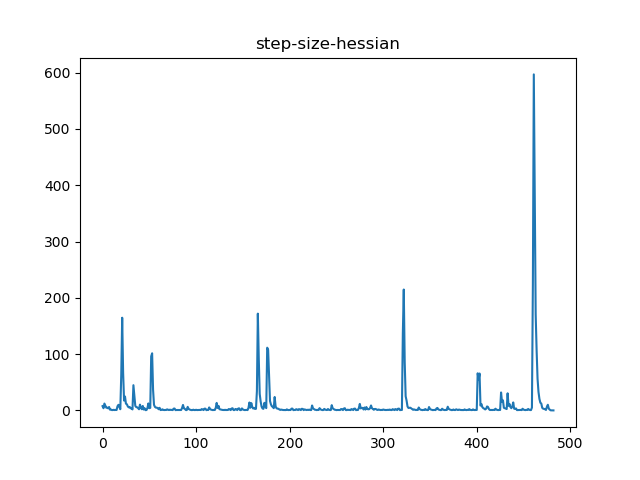
\includegraphics[width=.8\linewidth]{{c:/Users/julian/git/mdn/aufg2/step-size-hessian.png}}
	\end{center}
\end{frame}
\begin{frame}
\frametitle{Schrittweite für Quasi-Newton: BFGS}
	\begin{center}
		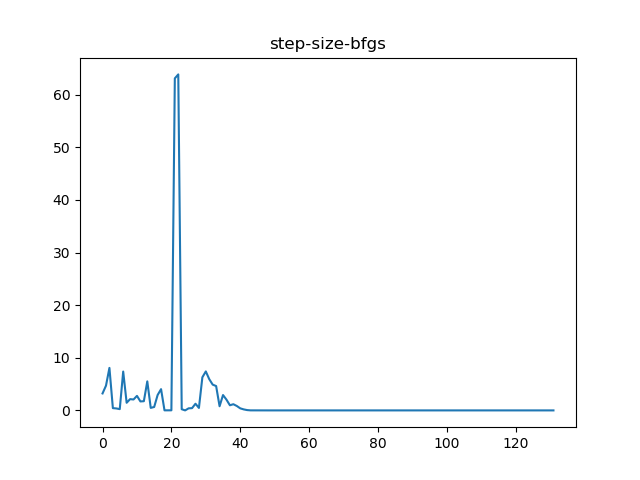
\includegraphics[width=.8\linewidth]{{c:/Users/julian/git/mdn/aufg2/step-size-bfgs.png}}
	\end{center}
\end{frame}
\begin{frame}
\frametitle{Schrittweite für Quasi-Newton: Broyden}
	\begin{center}
		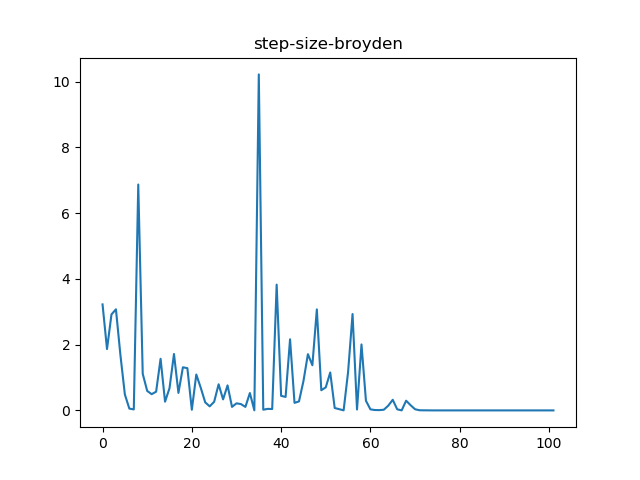
\includegraphics[width=.8\linewidth]{{c:/Users/julian/git/mdn/aufg2/step-size-broyden.png}}
	\end{center}
\end{frame}


\section{Aufgabe 3 - Norm}
\begin{frame}
\frametitle{Problemstellung}
	Sei
		$$A = \begin{pmatrix}
			1				& \frac{1}{2} 	& \frac{1}{4} 	& \frac{1}{7} 	& \\
			\frac{1}{3}		& \frac{1}{5}	& \frac{1}{8}	& 				& \\
			\frac{1}{6}		& \frac{1}{9}	&				& \ddots		& \\
			\frac{1}{10}	& 				& \ddots		&				& \\
		\end{pmatrix}$$
	Was ist $||A||_2$ auf $10$ signifikante Stellen genau?
\end{frame}
\begin{frame}
\frametitle{Allgemeines Lösungsverfahren}
	Es gilt nach Vorlesung $$||A_n||_2 \leq ||A_m||_2 \leq \lim_{k \to \infty} ||A_k||_2 = ||A||_2 \leq ||A||_F = \frac{\pi}{\sqrt{6}}$$
	mit $n \leq m$ und $A_n$ der linken oberen $n\times n$-Teilmatrix von $A$.

	Setze $B := A^T A$.
	
	$B$ ist symmetrisch und damit diagonalisierbar.

	Für den betragsgrößten Eigenwert $\lambda$ und seinen Eigenvektor $v$ gilt $Bv = \lambda v$ und, da $B$ diagonalisierbar
	$||Bv||_2 = ||B||_2 \cdot ||v||_2$, insgesamt



\end{frame}
\begin{frame}
\frametitle{Untere Grenze}
	$$||A_n||_2 = \sqrt{\rho(A_n^T A_n)} = \sqrt{\rho(B)} \quad \forall n \in \mathbb{N}$$
	
	Berechne diese untere Grenze für ein $n$:
	
	Das von-Mises-Verfahren liefert schnell eine Abschätzung an den betragsgrößten Eigenwert von $B$ und gibt auch den dazugehörigen Eigenvektor $v$ zurück.


\end{frame}
\begin{frame}
\frametitle{Obere Grenze}
	Der Eigenvektor $v$, den man aus dem von-Mises-Verfahren erhält, ist normiert und hat nur positive Einträge. Außerdem sind die Einträge mit steigendem Index monoton fallend.

	Erweitere diesen Vektor nun auf $m$ Dimensionen, indem für die Einträge $v_n+1, v_n+2, ..., v_m$ der Wert von $v_n$ angenommen wird und nenne ihn $v'$.
	
	Berechne dann $A_m^T A_m v' = B v'$
	
	Dies liefert eine obere Grenze von $||A||_2$
\end{frame}

\begin{frame}
\frametitle{Lösung}
	\footnotesize
	\begin{tabular}{l|l|l|l|l}
		$n$ 	& $m$ 		& von Mises 			& Eigenvektoren			& Ergebnis			\\ \hline \hline
		$8000$ 	& $10000$	& $1.2742241528116438$	&$1.2742241528249134$	&$1.2742241528$	\\
		$8000$	& $16000$	& $1.2742241528116438$	&$1.2742241528221396$	&$1.2742241528$	\\
		$12000$	& $24000$	& $1.2742241528182108$	&$1.2742241528211977$ 	&$1.2742241528$
		
	\end{tabular}
	\normalsize
\end{frame}


\end{document}